%----------------------------------------
\begin{frame}
  \frametitle{}

\begin{center}
{\Large\bf Questions?}

\vspace{1.0cm}

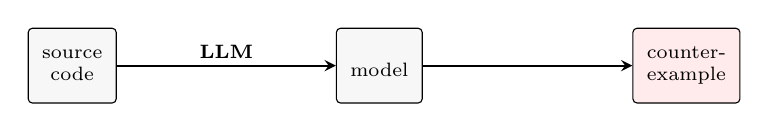
\begin{tikzpicture}[
  font=\scriptsize, >=stealth,
  box/.style={draw, rounded corners=1.5pt, align=center, inner sep=5pt,
              minimum height=0.95cm, fill=black!3},
  lab/.style={font=\scriptsize\bfseries, inner sep=2pt}
]
  \node[box] (code)  at (0,0)    {source\\code};
  \node[box] (model) at (3.9,0)  {\promelaname{}\\model};
  \node[box, fill=red!8] (cex) at (7.8,0) {counter-\\example};

  \draw[->, thick] (code)  -- node[lab, above] {LLM}    (model);
  \draw[->, thick] (model) -- node[lab, above] {\spin{}} (cex);
\end{tikzpicture}

\vspace{1.6cm}

{\normalsize \url{https://spinroot.com}}
\end{center}

\end{frame}
